\chapter{WARPLab 7.4 Modifications for WURC}
\label{sec_warplab_arch}

Here, we present a generated diagram mapping the entire WARPLab Version 7.4 \cite{warplab} software architecture hierarchy of function calls and highlighting the calls that needed to be modified to support the WURC \ac{PHY}.

Function calls with \textbf{blue} titles in Figure~\ref{fig_warplab_arch} were untouched, where as functions calls with \textbf{purple} labels had to be modified to extend their functionality.

For example: operations like {IFC\_CHANNEL}: would need to be augmented to extend the WARPLab supported channels to UHF channels.

We extended the WARPLab Node object with a new \texttt{wsd\_node} object that called into overridden MATLAB functions.
WARPLab scripts that wished to utilize WARPv3 board augmented with WURC would initialize them as \texttt{wsd\_nodes} and generally follow the same procedures as before.
Finally, we wrote WARPLab \acp{API} to directly execute arbitrary \ac{WURC} macros, including raw register read/write operations on the LMS6002D register map, providing full access to WARPLab experimental scripts.

% WURC block diagram
\begin{figure}[p]
\centering
  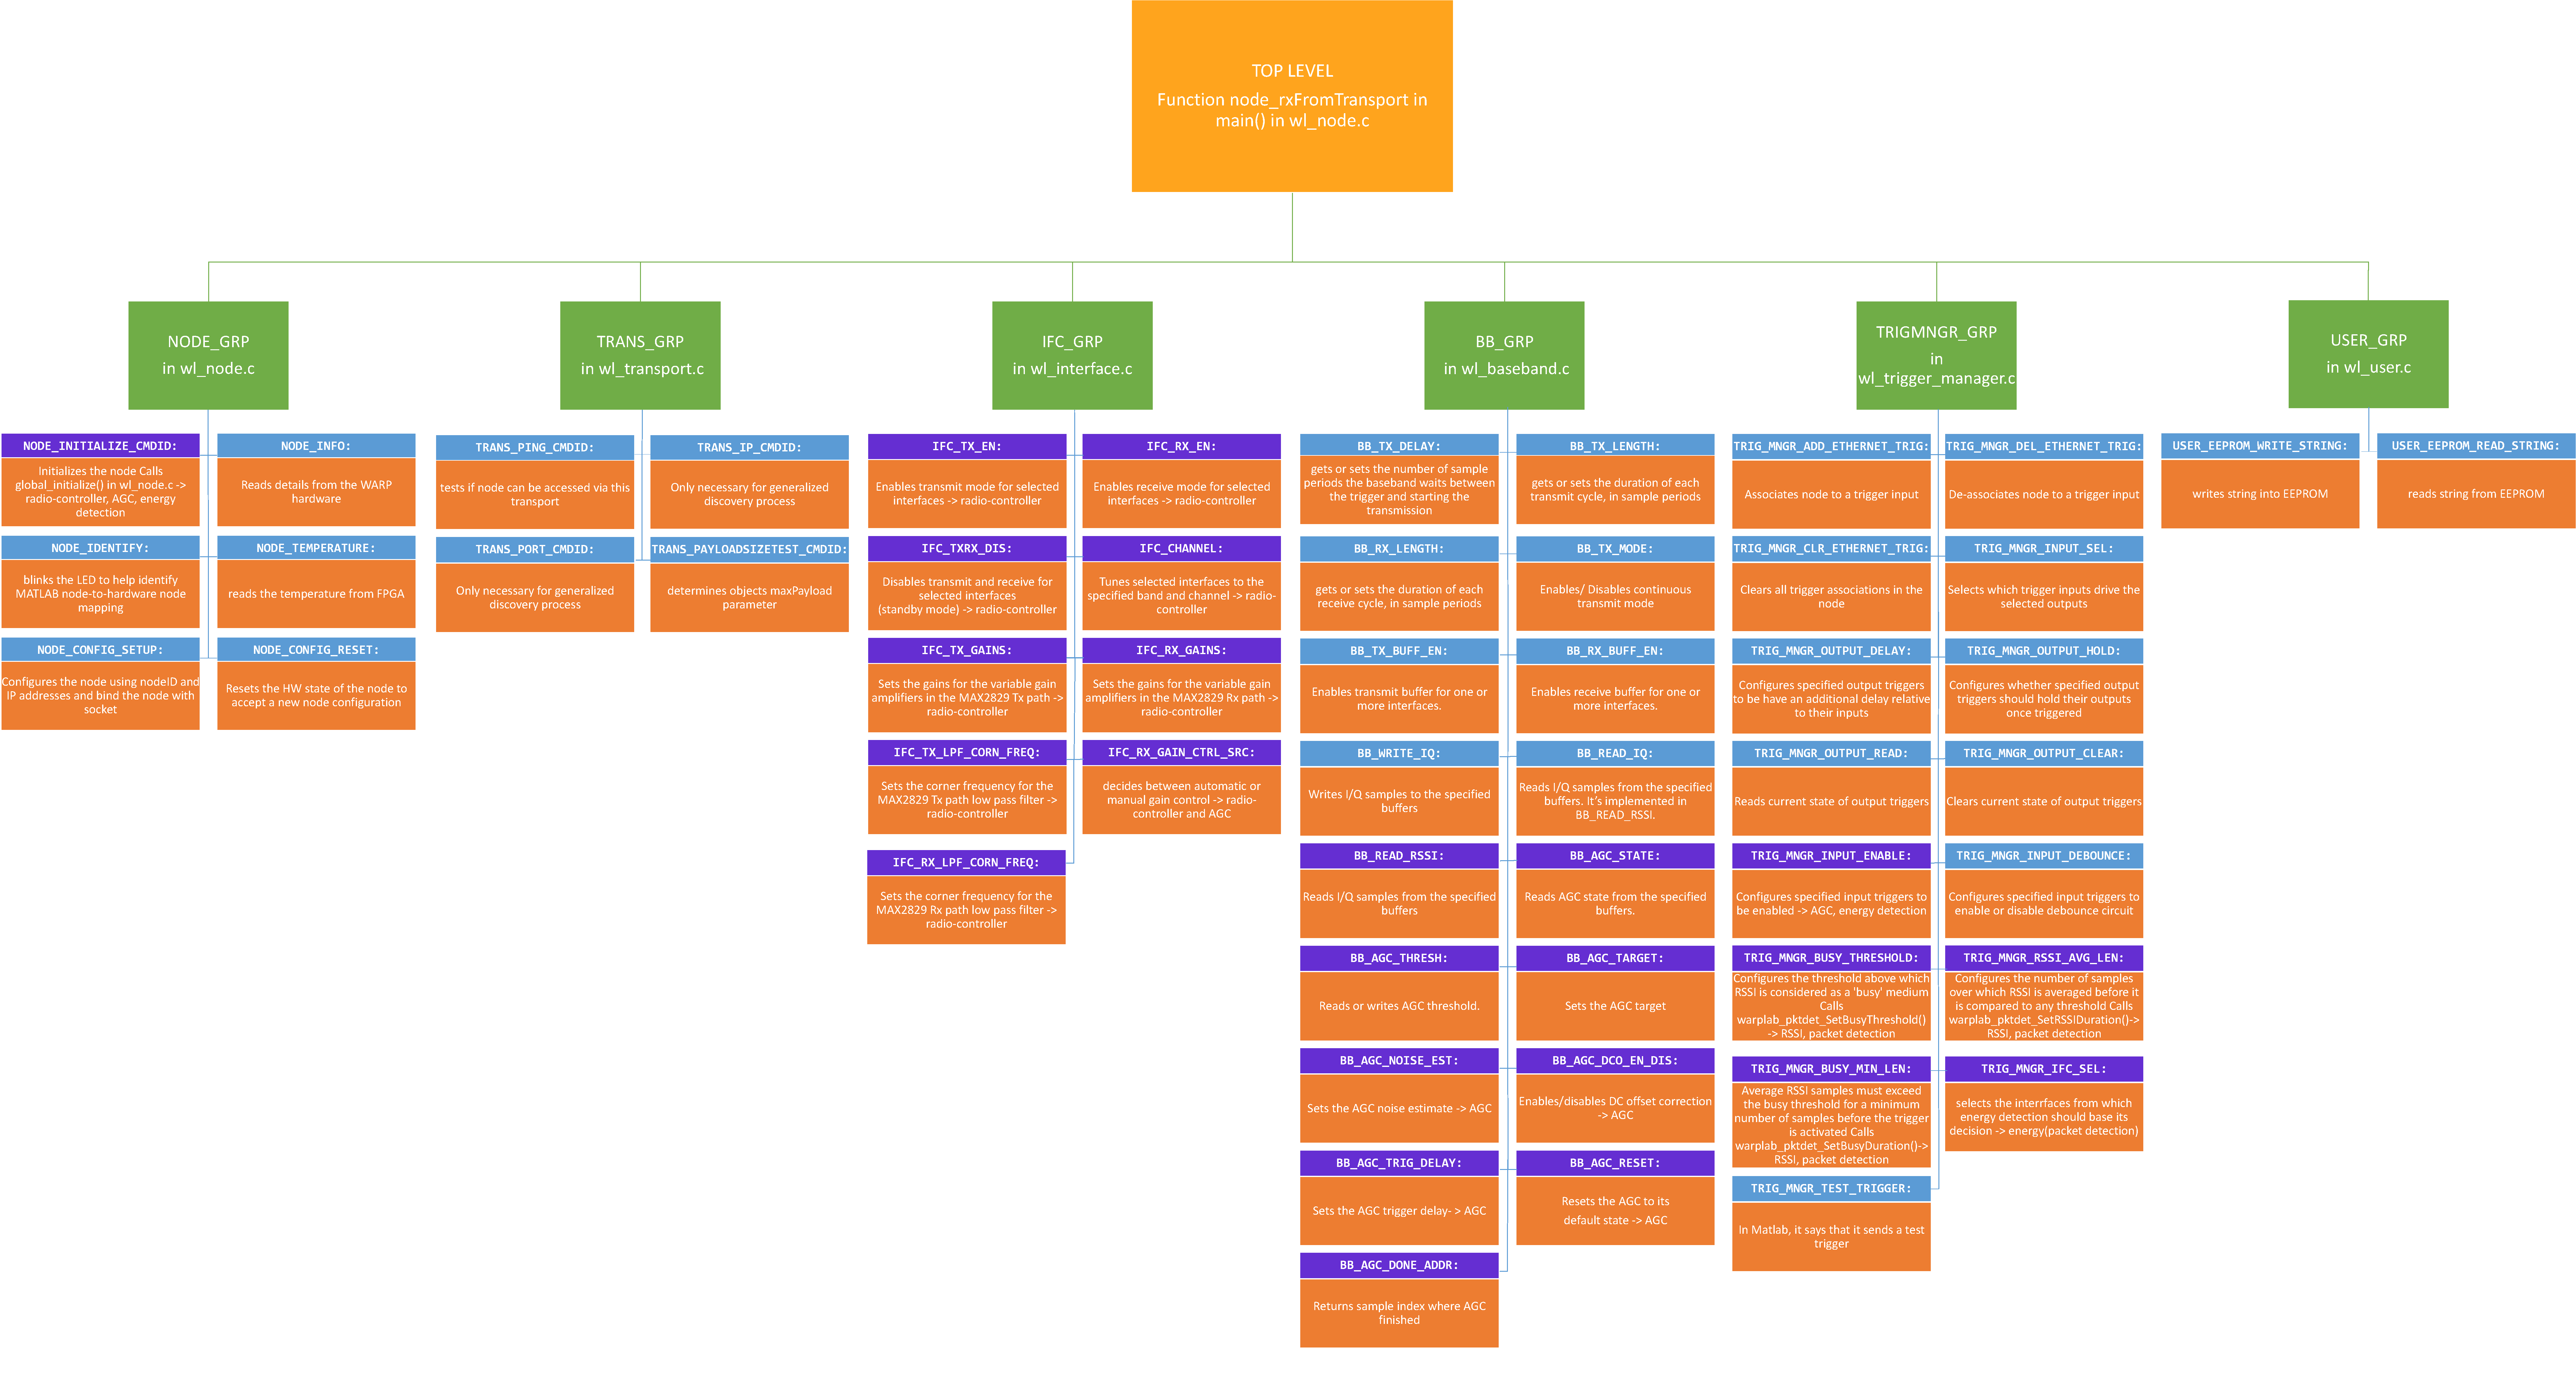
\includegraphics[width=1.4\linewidth, angle=270,origin=c]{figs/wurc/wurc_warplab_final_tree_v7p4}   
    \caption{WURC/WARPLab Software Architecture Diagram}
\label{fig_warplab_arch}
\end{figure}



%\section{WARP MicroBlaze Console API}
%
%\begin{singlespace}
%\small
%\begin{verbatim}
%
%TODO
%
%\end{verbatim}
%\end{singlespace}